% shared preamble of the theory figures (white background, purple / black theme, sans-serif)
\documentclass[tikz,border=8pt]{standalone}
\usepackage[T1]{fontenc}
\usepackage[scaled=0.92]{helvet}
\renewcommand{\familydefault}{\sfdefault}
\usepackage{amsmath,amssymb}
\usepackage[helvet]{sfmath}
\usetikzlibrary{arrows.meta,calc,decorations.pathreplacing,positioning,backgrounds}
\definecolor{ink}{HTML}{1A1A1F}
\definecolor{cohesin}{HTML}{6A3DE8}
\definecolor{condensin}{HTML}{1BAF7A}
\definecolor{fwd}{HTML}{D1303F}      % CTCF pointing right
\definecolor{rev}{HTML}{2B62D9}      % CTCF pointing left
\definecolor{panel}{HTML}{F8F6FD}
\definecolor{panelline}{HTML}{E3DDF5}
\tikzset{
  fiber/.style={line width=2.1pt,ink,line cap=round,line join=round},
  halo/.style={line width=6pt,white,line cap=round},
  lab/.style={font=\small,text=ink},
  note/.style={font=\footnotesize,text=ink!60},
  hd/.style={font=\bfseries\small,text=ink,anchor=west},
  leader/.style={line width=0.6pt,ink!45},
}
% soft panel, numbered badge, heading
\newcommand{\panelbg}[4]{\draw[rounded corners=9pt,fill=panel,draw=panelline,line width=0.9pt] (#1,#2) rectangle (#3,#4);}
\newcommand{\badge}[3]{\fill[ink] (#1,#2) circle (0.21);\node[white,font=\bfseries\footnotesize] at (#1,#2) {#3};}
% CTCF: a protein on the fibre carrying an arrow that gives the motif direction (f = right, r = left)
\newcommand{\protf}[2]{\draw[rounded corners=3.5pt,line width=0.6pt,draw=fwd!65!black,fill=fwd] (#1-0.3,#2-0.19) rectangle (#1+0.3,#2+0.19);
  \draw[white,line width=1.5pt,-{Stealth[length=3.4pt,width=4.4pt]}] (#1-0.15,#2)--(#1+0.16,#2);}
\newcommand{\protr}[2]{\draw[rounded corners=3.5pt,line width=0.6pt,draw=rev!65!black,fill=rev] (#1-0.3,#2-0.19) rectangle (#1+0.3,#2+0.19);
  \draw[white,line width=1.5pt,-{Stealth[length=3.4pt,width=4.4pt]}] (#1+0.15,#2)--(#1-0.16,#2);}
\newcommand{\prot}[3]{\csname prot#3\endcsname{#1}{#2}}
% ring seen at an angle, drawn as a tube (dark outline, light core); back half and front half
\newcommand{\ringpart}[5]{\draw[line width=4.6pt,#3!80!black,line cap=round] ([shift={(#1,#2)}]#4:0.55 and 0.21) arc[start angle=#4,end angle=#5,x radius=0.55,y radius=0.21];
  \draw[line width=2.4pt,#3!55!white,line cap=round] ([shift={(#1,#2)}]#4:0.55 and 0.21) arc[start angle=#4,end angle=#5,x radius=0.55,y radius=0.21];}
\newcommand{\ringback}[3]{\ringpart{#1}{#2}{#3}{180}{0}}
\newcommand{\ringfront}[3]{\ringpart{#1}{#2}{#3}{180}{360}}
% smooth loop whose foot (ring) is at (cx,y0): half-width W, height H, ring colour
\newcommand{\lloop}[5]{%
  \ringback{#1}{#2}{#5}%
  \draw[fiber] (#1-0.3,#2) .. controls (#1-0.3,#2+0.25*#4) and (#1-#3,#2+0.2*#4) .. (#1-#3,#2+0.55*#4)
     .. controls (#1-#3,#2+0.95*#4) and (#1-0.5*#3,#2+#4) .. (#1,#2+#4)
     .. controls (#1+0.5*#3,#2+#4) and (#1+#3,#2+0.95*#4) .. (#1+#3,#2+0.55*#4)
     .. controls (#1+#3,#2+0.2*#4) and (#1+0.3,#2+0.25*#4) .. (#1+0.3,#2);%
  \ringfront{#1}{#2}{#5}}
% gently undulating fibre from x0 to the loop foot at cx (height y0), and from x1
\newcommand{\base}[4]{%
  \draw[fiber] plot[smooth] coordinates {(#1,0.05) (#1+0.35*#3-0.35*#1,-0.05) (#3-1.4,0.04)} .. controls (#3-0.6,0.02) and (#3-0.3,0.05) .. (#3-0.3,#4);
  \draw[fiber] plot[smooth] coordinates {(#2,-0.05) (#2-0.35*#2+0.35*#3,0.05) (#3+1.4,-0.04)} .. controls (#3+0.6,-0.02) and (#3+0.3,0.05) .. (#3+0.3,#4);}
% stop sign for a blocked leg and a leg arrow
\newcommand{\stopbar}[3]{\draw[#3,line width=2.4pt,line cap=round] (#1,#2-0.2)--(#1,#2+0.2);}
\newcommand{\legarrow}[3]{\draw[cohesin,line width=1.6pt,-{Stealth[length=5pt,width=6pt]},line cap=round] (#1,#3)--(#2,#3);}

\definecolor{A}{HTML}{D1303F}\definecolor{B}{HTML}{5B4FD6}
\tikzset{ln/.style={line width=0.7pt,ink!45},cur/.style={line width=1.8pt,cohesin},thin/.style={line width=0.9pt},
  mv/.style={line width=1.2pt,ink!70,-{Stealth[length=5pt,width=6pt]}},box/.style={rounded corners=5pt,draw=cohesin!70,fill=white,line width=0.9pt,align=center,font=\small,text=ink,inner sep=4pt}}
\begin{document}
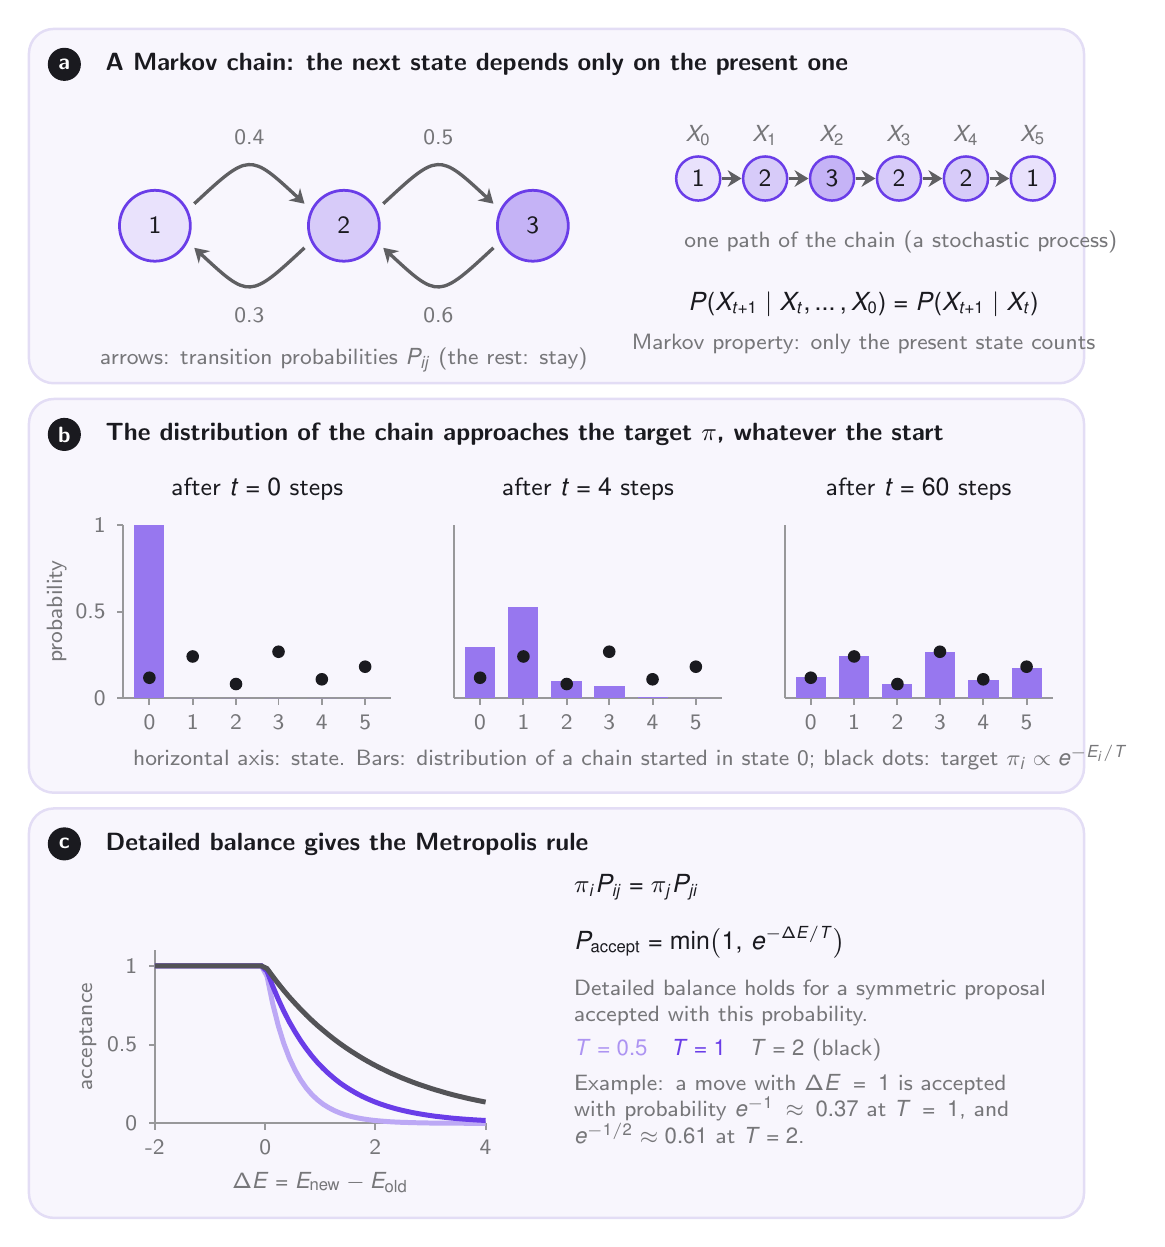
\begin{tikzpicture}
  \panelbg{0}{8.9}{13.4}{13.4}\badge{0.45}{12.950000000000001}{a}\node[hd] at (0.85,12.950000000000001) {A Markov chain: the next state depends only on the present one};
  \panelbg{0}{3.7}{13.4}{8.7}\badge{0.45}{8.25}{b}\node[hd] at (0.85,8.25) {The distribution of the chain approaches the target $\pi$, whatever the start};
  \panelbg{0}{-1.7}{13.4}{3.5}\badge{0.45}{3.05}{c}\node[hd] at (0.85,3.05) {Detailed balance gives the Metropolis rule};
  \fill[cohesin!15] (1.6,10.9) circle (0.45);\draw[cohesin,line width=1pt] (1.6,10.9) circle (0.45);\node[lab] at (1.6,10.9) {1};
  \fill[cohesin!27] (4.0,10.9) circle (0.45);\draw[cohesin,line width=1pt] (4.0,10.9) circle (0.45);\node[lab] at (4.0,10.9) {2};
  \fill[cohesin!39] (6.4,10.9) circle (0.45);\draw[cohesin,line width=1pt] (6.4,10.9) circle (0.45);\node[lab] at (6.4,10.9) {3};
  \draw[mv] (2.10,11.18) .. controls (2.80,11.83) .. (3.50,11.18);\node[note] at (2.80,12.03) {0.4};
  \draw[mv] (3.50,10.62) .. controls (2.80,9.97) .. (2.10,10.62);\node[note] at (2.80,9.77) {0.3};
  \draw[mv] (4.50,11.18) .. controls (5.20,11.83) .. (5.90,11.18);\node[note] at (5.20,12.03) {0.5};
  \draw[mv] (5.90,10.62) .. controls (5.20,9.97) .. (4.50,10.62);\node[note] at (5.20,9.77) {0.6};
  \node[note] at (4.0,9.2) {arrows: transition probabilities $P_{ij}$ (the rest: stay)};
  \fill[cohesin!15] (8.50,11.5) circle (0.28);\draw[cohesin,line width=0.9pt] (8.50,11.5) circle (0.28);\node[lab] at (8.50,11.5) {1};
  \node[note] at (8.50,12.05) {$X_{0}$};
  \fill[cohesin!27] (9.35,11.5) circle (0.28);\draw[cohesin,line width=0.9pt] (9.35,11.5) circle (0.28);\node[lab] at (9.35,11.5) {2};
  \node[note] at (9.35,12.05) {$X_{1}$};
  \draw[mv] (8.80,11.5)--(9.05,11.5);
  \fill[cohesin!39] (10.20,11.5) circle (0.28);\draw[cohesin,line width=0.9pt] (10.20,11.5) circle (0.28);\node[lab] at (10.20,11.5) {3};
  \node[note] at (10.20,12.05) {$X_{2}$};
  \draw[mv] (9.65,11.5)--(9.90,11.5);
  \fill[cohesin!27] (11.05,11.5) circle (0.28);\draw[cohesin,line width=0.9pt] (11.05,11.5) circle (0.28);\node[lab] at (11.05,11.5) {2};
  \node[note] at (11.05,12.05) {$X_{3}$};
  \draw[mv] (10.50,11.5)--(10.75,11.5);
  \fill[cohesin!27] (11.90,11.5) circle (0.28);\draw[cohesin,line width=0.9pt] (11.90,11.5) circle (0.28);\node[lab] at (11.90,11.5) {2};
  \node[note] at (11.90,12.05) {$X_{4}$};
  \draw[mv] (11.35,11.5)--(11.60,11.5);
  \fill[cohesin!15] (12.75,11.5) circle (0.28);\draw[cohesin,line width=0.9pt] (12.75,11.5) circle (0.28);\node[lab] at (12.75,11.5) {1};
  \node[note] at (12.75,12.05) {$X_{5}$};
  \draw[mv] (12.20,11.5)--(12.45,11.5);
  \node[note,anchor=west] at (8.2,10.7) {one path of the chain (a stochastic process)};
  \node[lab] at (10.6,9.9) {$P(X_{t+1}\mid X_t,\dots,X_0)=P(X_{t+1}\mid X_t)$};
  \node[note] at (10.6,9.4) {Markov property: only the present state counts};
  \draw[ln] (1.2,4.9)--(4.6,4.9);\draw[ln] (1.2,4.9)--(1.2,7.1000000000000005);
  \draw[ln] (1.53,4.9)--(1.53,4.82);\node[note] at (1.53,4.6000000000000005) {0};
  \draw[ln] (2.08,4.9)--(2.08,4.82);\node[note] at (2.08,4.6000000000000005) {1};
  \draw[ln] (2.63,4.9)--(2.63,4.82);\node[note] at (2.63,4.6000000000000005) {2};
  \draw[ln] (3.17,4.9)--(3.17,4.82);\node[note] at (3.17,4.6000000000000005) {3};
  \draw[ln] (3.72,4.9)--(3.72,4.82);\node[note] at (3.72,4.6000000000000005) {4};
  \draw[ln] (4.27,4.9)--(4.27,4.82);\node[note] at (4.27,4.6000000000000005) {5};
  \draw[ln] (1.2,4.90)--(1.1199999999999999,4.90);\node[note,anchor=east] at (1.0999999999999999,4.90) {0};
  \draw[ln] (1.2,6.00)--(1.1199999999999999,6.00);\node[note,anchor=east] at (1.0999999999999999,6.00) {0.5};
  \draw[ln] (1.2,7.10)--(1.1199999999999999,7.10);\node[note,anchor=east] at (1.0999999999999999,7.10) {1};
  \node[note,rotate=90] at (0.35,6.00) {probability};
  \fill[cohesin!70] (1.337,4.900) rectangle (1.721,7.100);
  \fill[cohesin!70] (1.885,4.900) rectangle (2.269,4.900);
  \fill[cohesin!70] (2.434,4.900) rectangle (2.818,4.900);
  \fill[cohesin!70] (2.982,4.900) rectangle (3.366,4.900);
  \fill[cohesin!70] (3.531,4.900) rectangle (3.915,4.900);
  \fill[cohesin!70] (4.079,4.900) rectangle (4.463,4.900);
  \draw[line width=1.4pt,ink,only marks] plot coordinates {(1.529,5.165) (2.077,5.433) (2.626,5.078) (3.174,5.489) (3.723,5.140) (4.271,5.295)};
  \fill[ink] (1.53,5.16) circle (0.08);
  \fill[ink] (2.08,5.43) circle (0.08);
  \fill[ink] (2.63,5.08) circle (0.08);
  \fill[ink] (3.17,5.49) circle (0.08);
  \fill[ink] (3.72,5.14) circle (0.08);
  \fill[ink] (4.27,5.30) circle (0.08);
  \node[lab] at (2.90,7.55) {after $t=0$ steps};
  \draw[ln] (5.4,4.9)--(8.8,4.9);\draw[ln] (5.4,4.9)--(5.4,7.1000000000000005);
  \draw[ln] (5.73,4.9)--(5.73,4.82);\node[note] at (5.73,4.6000000000000005) {0};
  \draw[ln] (6.28,4.9)--(6.28,4.82);\node[note] at (6.28,4.6000000000000005) {1};
  \draw[ln] (6.83,4.9)--(6.83,4.82);\node[note] at (6.83,4.6000000000000005) {2};
  \draw[ln] (7.37,4.9)--(7.37,4.82);\node[note] at (7.37,4.6000000000000005) {3};
  \draw[ln] (7.92,4.9)--(7.92,4.82);\node[note] at (7.92,4.6000000000000005) {4};
  \draw[ln] (8.47,4.9)--(8.47,4.82);\node[note] at (8.47,4.6000000000000005) {5};
  \fill[cohesin!70] (5.537,4.900) rectangle (5.921,5.552);
  \fill[cohesin!70] (6.085,4.900) rectangle (6.469,6.057);
  \fill[cohesin!70] (6.634,4.900) rectangle (7.018,5.114);
  \fill[cohesin!70] (7.182,4.900) rectangle (7.566,5.058);
  \fill[cohesin!70] (7.731,4.900) rectangle (8.115,4.919);
  \fill[cohesin!70] (8.279,4.900) rectangle (8.663,4.900);
  \draw[line width=1.4pt,ink,only marks] plot coordinates {(5.729,5.165) (6.277,5.433) (6.826,5.078) (7.374,5.489) (7.923,5.140) (8.471,5.295)};
  \fill[ink] (5.73,5.16) circle (0.08);
  \fill[ink] (6.28,5.43) circle (0.08);
  \fill[ink] (6.83,5.08) circle (0.08);
  \fill[ink] (7.37,5.49) circle (0.08);
  \fill[ink] (7.92,5.14) circle (0.08);
  \fill[ink] (8.47,5.30) circle (0.08);
  \node[lab] at (7.10,7.55) {after $t=4$ steps};
  \draw[ln] (9.6,4.9)--(13.0,4.9);\draw[ln] (9.6,4.9)--(9.6,7.1000000000000005);
  \draw[ln] (9.93,4.9)--(9.93,4.82);\node[note] at (9.93,4.6000000000000005) {0};
  \draw[ln] (10.48,4.9)--(10.48,4.82);\node[note] at (10.48,4.6000000000000005) {1};
  \draw[ln] (11.03,4.9)--(11.03,4.82);\node[note] at (11.03,4.6000000000000005) {2};
  \draw[ln] (11.57,4.9)--(11.57,4.82);\node[note] at (11.57,4.6000000000000005) {3};
  \draw[ln] (12.12,4.9)--(12.12,4.82);\node[note] at (12.12,4.6000000000000005) {4};
  \draw[ln] (12.67,4.9)--(12.67,4.82);\node[note] at (12.67,4.6000000000000005) {5};
  \fill[cohesin!70] (9.737,4.900) rectangle (10.121,5.170);
  \fill[cohesin!70] (10.285,4.900) rectangle (10.669,5.442);
  \fill[cohesin!70] (10.834,4.900) rectangle (11.218,5.078);
  \fill[cohesin!70] (11.382,4.900) rectangle (11.766,5.485);
  \fill[cohesin!70] (11.931,4.900) rectangle (12.315,5.137);
  \fill[cohesin!70] (12.479,4.900) rectangle (12.863,5.288);
  \draw[line width=1.4pt,ink,only marks] plot coordinates {(9.929,5.165) (10.477,5.433) (11.026,5.078) (11.574,5.489) (12.123,5.140) (12.671,5.295)};
  \fill[ink] (9.93,5.16) circle (0.08);
  \fill[ink] (10.48,5.43) circle (0.08);
  \fill[ink] (11.03,5.08) circle (0.08);
  \fill[ink] (11.57,5.49) circle (0.08);
  \fill[ink] (12.12,5.14) circle (0.08);
  \fill[ink] (12.67,5.30) circle (0.08);
  \node[lab] at (11.30,7.55) {after $t=60$ steps};
  \node[note,anchor=west] at (1.2,4.15) {horizontal axis: state. Bars: distribution of a chain started in state 0; black dots: target $\pi_i\propto e^{-E_i/T}$};
  \draw[ln] (1.6,-0.5)--(5.800000000000001,-0.5);\draw[ln] (1.6,-0.5)--(1.6,1.7000000000000002);
  \draw[ln] (1.60,-0.5)--(1.60,-0.58);\node[note] at (1.60,-0.8) {-2};
  \draw[ln] (3.00,-0.5)--(3.00,-0.58);\node[note] at (3.00,-0.8) {0};
  \draw[ln] (4.40,-0.5)--(4.40,-0.58);\node[note] at (4.40,-0.8) {2};
  \draw[ln] (5.80,-0.5)--(5.80,-0.58);\node[note] at (5.80,-0.8) {4};
  \draw[ln] (1.6,-0.50)--(1.52,-0.50);\node[note,anchor=east] at (1.5,-0.50) {0};
  \draw[ln] (1.6,0.50)--(1.52,0.50);\node[note,anchor=east] at (1.5,0.50) {0.5};
  \draw[ln] (1.6,1.50)--(1.52,1.50);\node[note,anchor=east] at (1.5,1.50) {1};
  \node[note] at (3.70,-1.25) {$\Delta E=E_{\mathrm{new}}-E_{\mathrm{old}}$};
  \node[note,rotate=90] at (0.75,0.60) {acceptance};
  \draw[line width=1.8pt,cohesin!45] plot coordinates {(1.600,1.500) (1.671,1.500) (1.742,1.500) (1.814,1.500) (1.885,1.500) (1.956,1.500) (2.027,1.500) (2.098,1.500) (2.169,1.500) (2.241,1.500) (2.312,1.500) (2.383,1.500) (2.454,1.500) (2.525,1.500) (2.597,1.500) (2.668,1.500) (2.739,1.500) (2.810,1.500) (2.881,1.500) (2.953,1.500) (3.024,1.369) (3.095,1.025) (3.166,0.744) (3.237,0.515) (3.308,0.328) (3.380,0.176) (3.451,0.052) (3.522,-0.050) (3.593,-0.133) (3.664,-0.200) (3.736,-0.256) (3.807,-0.300) (3.878,-0.337) (3.949,-0.367) (4.020,-0.392) (4.092,-0.412) (4.163,-0.428) (4.234,-0.441) (4.305,-0.452) (4.376,-0.461) (4.447,-0.468) (4.519,-0.474) (4.590,-0.479) (4.661,-0.483) (4.732,-0.486) (4.803,-0.488) (4.875,-0.491) (4.946,-0.492) (5.017,-0.494) (5.088,-0.495) (5.159,-0.496) (5.231,-0.497) (5.302,-0.497) (5.373,-0.498) (5.444,-0.498) (5.515,-0.498) (5.586,-0.499) (5.658,-0.499) (5.729,-0.499) (5.800,-0.499)};
  \draw[line width=1.8pt,cohesin] plot coordinates {(1.600,1.500) (1.671,1.500) (1.742,1.500) (1.814,1.500) (1.885,1.500) (1.956,1.500) (2.027,1.500) (2.098,1.500) (2.169,1.500) (2.241,1.500) (2.312,1.500) (2.383,1.500) (2.454,1.500) (2.525,1.500) (2.597,1.500) (2.668,1.500) (2.739,1.500) (2.810,1.500) (2.881,1.500) (2.953,1.500) (3.024,1.433) (3.095,1.246) (3.166,1.078) (3.237,0.925) (3.308,0.787) (3.380,0.663) (3.451,0.550) (3.522,0.449) (3.593,0.357) (3.664,0.274) (3.736,0.199) (3.807,0.132) (3.878,0.071) (3.949,0.015) (4.020,-0.034) (4.092,-0.079) (4.163,-0.120) (4.234,-0.157) (4.305,-0.190) (4.376,-0.220) (4.447,-0.247) (4.519,-0.272) (4.590,-0.294) (4.661,-0.314) (4.732,-0.332) (4.803,-0.348) (4.875,-0.363) (4.946,-0.376) (5.017,-0.388) (5.088,-0.399) (5.159,-0.409) (5.231,-0.417) (5.302,-0.425) (5.373,-0.433) (5.444,-0.439) (5.515,-0.445) (5.586,-0.450) (5.658,-0.455) (5.729,-0.459) (5.800,-0.463)};
  \draw[line width=1.8pt,ink!75] plot coordinates {(1.600,1.500) (1.671,1.500) (1.742,1.500) (1.814,1.500) (1.885,1.500) (1.956,1.500) (2.027,1.500) (2.098,1.500) (2.169,1.500) (2.241,1.500) (2.312,1.500) (2.383,1.500) (2.454,1.500) (2.525,1.500) (2.597,1.500) (2.668,1.500) (2.739,1.500) (2.810,1.500) (2.881,1.500) (2.953,1.500) (3.024,1.466) (3.095,1.369) (3.166,1.276) (3.237,1.188) (3.308,1.104) (3.380,1.025) (3.451,0.949) (3.522,0.877) (3.593,0.809) (3.664,0.744) (3.736,0.683) (3.807,0.624) (3.878,0.568) (3.949,0.515) (4.020,0.465) (4.092,0.417) (4.163,0.372) (4.234,0.328) (4.305,0.287) (4.376,0.248) (4.447,0.211) (4.519,0.176) (4.590,0.142) (4.661,0.111) (4.732,0.080) (4.803,0.052) (4.875,0.024) (4.946,-0.002) (5.017,-0.026) (5.088,-0.050) (5.159,-0.072) (5.231,-0.093) (5.302,-0.114) (5.373,-0.133) (5.444,-0.151) (5.515,-0.168) (5.586,-0.185) (5.658,-0.200) (5.729,-0.215) (5.800,-0.229)};
  \node[lab,anchor=west] at (6.8,2.5) {$\pi_iP_{ij}=\pi_jP_{ji}$};\node[lab,anchor=west] at (6.8,1.8) {$P_{\mathrm{accept}}=\min\!\big(1,\,e^{-\Delta E/T}\big)$};\node[note,text width=6.0cm,anchor=north west] at (6.8,1.45) {Detailed balance holds for a symmetric proposal accepted with this probability.\\[3pt]\textcolor{cohesin!55}{$T=0.5$}\quad\textcolor{cohesin}{$T=1$}\quad $T=2$ (black)\\[3pt]Example: a move with $\Delta E=1$ is accepted with probability $e^{-1}\approx0.37$ at $T=1$, and $e^{-1/2}\approx0.61$ at $T=2$.};
\end{tikzpicture}
\end{document}
